%-------------------------
%minimal-unix
%(c) H.Buchmann FHNW 2014
%export TEXINPUTS=.:${HOME}/fhnw/edu/:${HOME}/fhnw/edu/tinL/config/latex:${HOME}/fhnw/edu/config//:
%-------------------------
\documentclass{beamer}
\usepackage{latex/beamer}
%---------------------
%local defines
%(c) H.Buchmann FHNW 2009
%$Id$
%---------------------
\newcommand{\target} {\beaglebone\xspace}
\newcommand{\targetS}{{\bf BBG}\xspace}
\newcommand{\host}   {{\em Host}\xspace}
\newcommand{\targetroot} {{\bf target-root}\xspace}
\newcommand{\kernel} {{\bf kernel}\xspace}
\renewcommand{\c}{{\bf C}\xspace}
\newcommand{\cpp}{{\bf C++}\xspace}
\newcommand{\posix}{{\bf POSIX}\xspace}

\input{/home/buchmann/latex/dirtree/dirtree.tex}

\usepackage[absolute]{textpos}
\setlength{\TPHorizModule}{1mm}
\setlength{\TPVertModule}{1mm}

\begin{document}

\newcommand{\qemu}{{\em qemu}\xspace}
\newcommand{\busybox}{{\em busybox}\xspace}
\newcommand{\yocto}{{\em yocto}\xspace}
\title{Zugriff auf die Hardware}

\frame{\titlepage}

\begin{frame}{Um was geht es ?}{Zugriff auf mehrere Arten}
 \begin{itemize}
  \item userspace
  \begin{itemize}
   \item per \cod{/sys/class/gpio}
   \item per \cod{mmap} mit eigenem Programm: 
  \end{itemize}
  \item kernelspace
  \begin{itemize}
   \item mit eigenem module
  \end{itemize}
 \end{itemize}
\end{frame}

\begin{frame}{{\em userspace} vs. {\em kernelspace}}{Systemcalls}
\begin{center}
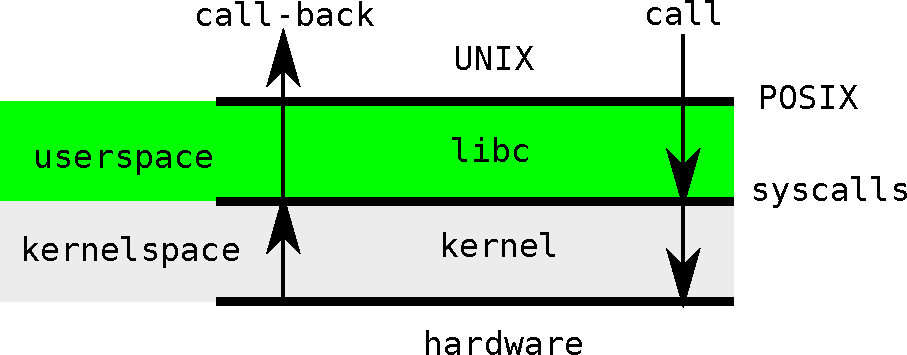
\includegraphics[width=10cm]{userspace-kernelspace.pdf}
\end{center}
\begin{description}[kernelspace]
 \item[userspace] geschützt, limitierte Zugriffsmöglichkeiten
 \item[kernelspace] ungeschützt, unlimitierte Zugriffsmöglichkeiten
\end{description}
\end{frame}

\subsection{syscalls}
\begin{frame}[fragile]{Syscall aus {\em user} Sicht }{\src{syscall-c.c}}
 \begin{lstlisting}[basicstyle=\footnotesize]
 /* write(f,void* buffer,unsigned len) */
 char s[]="Hello World\n";
         /*01234567890 */
 syscall(4,0,s,12);  /* we are in userspace */
     /*  |------------------ code for write */
 \end{lstlisting}
\end{frame}

\begin{frame}{Verzeichnisstruktur}
\dirtree{%
.1 25-modules.
.2 config.
.2 tc \DTcomment{link to toolchain}.
.2 target \DTcomment{sshfs \targetS}.
.2 work.
}
\remark{Siehe auch 17-build}
\end{frame}

\subsection{Aufgaben}
\begin{frame}{Aufgaben}
 \begin{itemize}
  \item Systemcall für \host/\targetS mit \c und \cpp
 \end{itemize}
\end{frame}

\section{Kernelspace}
\begin{frame}{Files}
 \begin{itemize}
 \item dmesg
 \end{itemize}
\end{frame}

\subsection{printk}
\begin{frame}{printk}{Das {\em kernel printf}}
 \begin{itemize}
  \item Siehe \cod{6-modules/src/simple-module.c}
 \end{itemize}
\end{frame}

\subsection{strace}
\begin{frame}{\cod{strace}}
 \begin{itemize}
  \item \cod{strace} {\Huge gibt es} {\tiny nat�rlich} {\Huge nicht}
 \end{itemize}
\end{frame}


\subsection{gdb}
\begin{frame}{Zwei Rechner}{Host Target}
 \begin{tabular}{l||c|c|c||l}
  		&	Host	&	& Target\\
  \hline
  seriell	&\cod{/dev/ttyUSB0}	&$\leftrightarrow$& \cod{/dev/ttyS} &debug\\
  ethernet	&\cod{eth0}		&$\leftrightarrow$& \cod{eth0} &Bedienung\\
 \end{tabular}
 
 \remark{die serielle Schnittstelle kann nicht f�r die Bedienung gebraucht werden}
\end{frame}

\begin{frame}{Konfiguration}
 \begin{description}
  \item[Target] Kernel hacking $\to$ KGDB kernel debugger
  \item[Host] gdb f�r ARM
  \begin{description}[configuration]
   \item[download]  \url{www.gnu.org/software/gdb/}
   \item[configuration]
    \cod{configure --prefix={\em where-on-host} $\backslash$\\
     --target=arm-none-linux-gnueabi}
  \end{description}
 \end{description}
\end{frame}

\begin{frame}{Anwendung}
 \begin{itemize}
  \item Siehe \url{DocBook/index.html} kgdb
 \end{itemize}
\end{frame}


\end{document}
